\documentclass[tikz]{standalone}
\usepackage{amsmath,amssymb}
\usepackage{pgfplots,multicol}

\pgfplotsset{compat=1.13}
\usepgfplotslibrary{fillbetween}

\begin{document}


 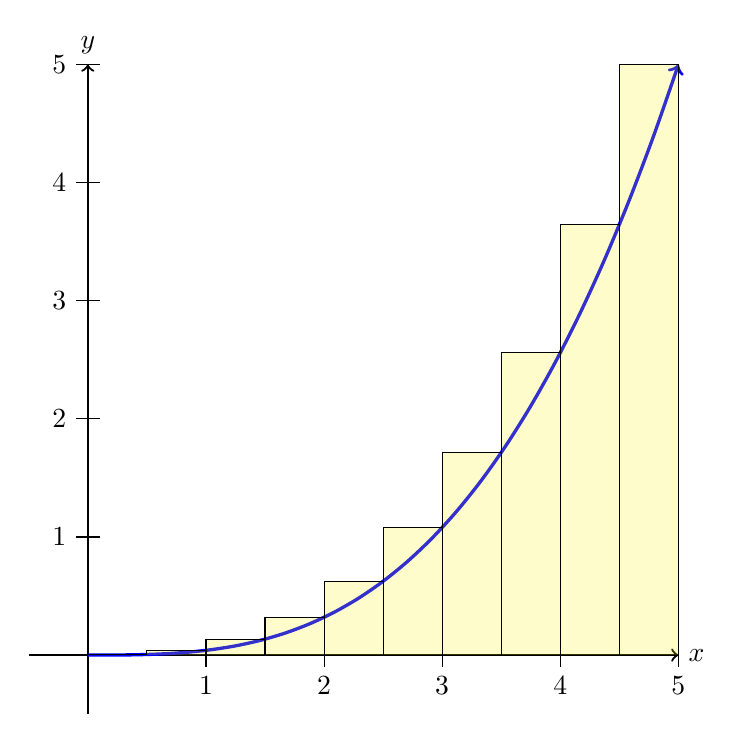
\begin{tikzpicture}[scale=1.5,	declare function={ f(\x) = 1/25*\x*\x*\x; 
                 }]
        \draw[->,thick] (-0.5,0) -- (5,0) node[right] {$x$};
    \draw[->,thick] (0,-0.5) -- (0,5) node[above] {$y$};
	\foreach \x in {1,2,3,4,5} \draw (\x,0.1) -- (\x, -0.1) node[below] {\x};
	\foreach \y in {1,2,3,4,5} \draw (0.1,\y) -- (-0.1, \y) node[left] {\y};
	\draw[->,smooth,domain=0:5,very thick,blue] plot(\x,{f(\x)});
	

\foreach \t in {0,0.5,1,1.5,2,2.5,3,3.5,4,4.5} \draw[fill=yellow, fill opacity=0.2] (\t,0) -- (\t,{f(\t+0.5)}) -- ({\t+0.5}, {f(\t+0.5)}) -- ({\t+0.5},0);
	

\end{tikzpicture}

	
\end{document}
